\documentclass[10pt,handout,usenames,dvipsnames,pdf]{beamer}
% \documentclass[10pt,usenames,dvipsnames,pdf]{beamer}

\usepackage[portuguese,english]{babel}

\usepackage[backend=biber,style=authoryear-icomp,natbib=true,url=false,doi=true]{biblatex}

% \usepackage[notesposition=right,duration=20,lastminutes=5]{pdfpc}
\usepackage{appendixnumberbeamer}

\usepackage[scale=2]{ccicons}

\usepackage{hyperref}
\usepackage{booktabs}
\usepackage{multirow}
\usepackage{bookmark}

\usepackage[ruled,lined]{algorithm2e}
\usepackage{graphicx}
\usepackage{csquotes}
\usepackage{float}

\usepackage{pgfplots}
\usepackage{pgfgantt}

% Bibliography
\addbibresource{../references.bib}


% PDF Presenter Console (pdfpc) Notes
% \setbeamertemplate{note page}{\pagecolor{black!2}\normalsize\insertnote}

% \setbeameroption{hide notes}
% \setbeameroption{show notes on second screen=right}

\newcommand<>{\talknote}[1]{\only#2{\note[item]{\textbf{#1}}\relax}}

% PDF Metadata
\hypersetup{
 pdftitle = {Principled Modelling Of The Google Hash Code Problems For Metaheuristics},
 pdfauthor = {Pedro Miguel Duque Rodrigues},
 pdfsubject = {Master Thesis - Intermediate Defense Presentation},
 pdfkeywords = {Intelligent Systems, Modelling, Meta-Heuristics},
 pdfproducer = {Latex Beamer with hyperref},
 pdfcreator = {lualatex},
}

% Beamer Theme
\usetheme[progressbar=frametitle, background=light]{metropolis}
\metroset{block=fill}

% Title Page Settings
\title{Principled Modelling Of The Google Hash Code Problems For Meta-Heuristics}
\subtitle{Intermediate Defense}
\author{Pedro Rodrigues \vspace{0.1cm} \\ \tiny Alexandre B. Jesus \\ \and Carlos M. Fonseca \\} 
\date{\footnotesize January 2023}
\institute{University of Coimbra \\ Department of Informatics Engineering}

\begin{document}

\begin{frame}[noframenumbering, plain]
  \titlepage
  \talknote{Welcome the audience}
\end{frame}

\begin{frame}{Outline}
  \tableofcontents
\end{frame}

\section{Introduction}

\begin{frame}{Motivation}
  This work is related to both theoretical and practical aspects that
  arise from the analysis of real-world problems.

  The motivation behind this work relates to the answer to three key questions:
  \begin{itemize}
    \item Why The Google \alert{Hash Code} Problems~?
    \item Why (Principled) \alert{Modelling}~?
    \item Why \alert{Meta-Heuristics}~?
  \end{itemize}
\end{frame}

\begin{frame}{Why The Google Hash Code Problems~?}
  The \alert{Hash Code} programming competition is a yearly event that invites people
  from around the world to solve a challenging problem.

  The contestants participate in teams of 2 to 4 elements and have about 4 hours
  to come up with a solution.

  The challenges:
  \begin{itemize}
    \item Are complex problems inspired by engineering challenges.
    \item Resemble real-world scenarios.
    \item Are well formulated and can be solved to some extent in a short amount of time (4 hours).
  \end{itemize}
\end{frame}

\begin{frame}{Why (Principled) Modelling~?}
  \alert{Modelling} is the process of creating a simplified representation
  or approximation of a real-world system, process, or phenomenon.

  If this process is done in a principled way, it can be standardized in order to provide:
  \begin{itemize}
    \item A structured approach to problem-solving.
    \item A clear separation between problems and solvers.
  \end{itemize}

  A good model encodes information about:
  \begin{itemize}
    \item The particular problem instance parameters.
    \item The space of possible solutions.
    \item How solutions can be evaluated.
  \end{itemize}
\end{frame}

\begin{frame}{Why Meta-Heuristics~?}

  \alert{Meta-Heuristics} are methods that ``guide and intelligently combine subordinate
  heuristics for exploring and exploiting solutions in the search
  space''~(\cite{osman1996metaheuristics}).

  These methods have interesting properties:
  \begin{itemize}
    \item General-purpose, i.e. they can be applied to many problems.
    \item Can often find ``good'' solutions for hard problems quickly.
  \end{itemize}

\end{frame}

\begin{frame}{The ``Big Picture''}
  \begin{figure}[h]
    \centering
    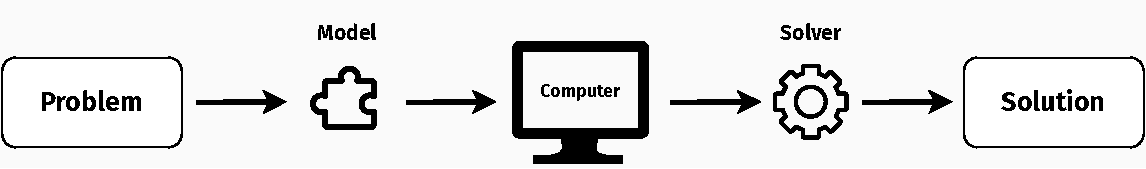
\includegraphics[width=\textwidth,keepaspectratio]{../assets/modelling/modelling-slides.pdf}
    \caption{Modelling and Problem-Solving}
  \end{figure}
\end{frame}

\section{Background}

\begin{frame}{Optimization}

  \begin{block}{Optimization Problem}
    An optimization problem is a collection $\mathcal{I}$ of instances,
    typically generated in a similar manner. An instance $\iota$ of an
    optimization problem consists of a pair $\left(\mathcal{S}, f\right)$, where
    $\mathcal{S}$ is a set containing all feasible solutions, and $f$ is an
    objective (cost) function such that:
    \begin{equation*}
      f \colon \mathcal{S} \longrightarrow \mathbb{R}
    \end{equation*}
  \end{block}

  \begin{block}{Combinatorial Optimization Problem}
    An instance $\iota$ of a combinatorial optimization problem is an instance of an
    optimization problem where the set $\mathcal{S}$ of feasible solutions is
    finite.
  \end{block}

\end{frame}

\begin{frame}{Global Optimization}
  \alert{Global Optimization} is the process of identifying a global optimal solution to
  a given optimization problem.

  \vspace{0.2cm}

  \begin{block}{Global Optimal Solution}
    Assuming, without loss of generality, the maximization of an objective
    function $f(s)$, a global optimal solution $s^*$ is expressed by:
    \begin{equation*}
      \forall s \in \mathcal{S} \colon f(s^{*}) \geq f(s)
    \end{equation*}
  \end{block}

\end{frame}

\begin{frame}{Local Optimization}
  \alert{Local Optimization} is the process of finding a solution that is
  optimal among those that are close to it in some sense.

  \vspace{0.2cm}

  \begin{block}{(Strictly) Local Optimal Solution}
    Assuming maximization without loss of generality, a solution $\hat{s}$ is
    locally optimal with respect to a given neighborhood structure $\mathcal{N}$
    iff:
    \begin{equation*}
      \forall s \in \mathcal{N}(\hat{s}) \colon f(\hat{s}) \geq f(s)
    \end{equation*}
    Furthermore, $\hat{s}$ is considered strictly locally optimal iff:
    \begin{equation*}
      \forall s \in \mathcal{N}(\hat{s}) \setminus \{\hat{s}\} \colon f(\hat{s}) > f(s)
    \end{equation*}
  \end{block}
\end{frame}

\begin{frame}{Example --- Global and Local Optimal Solutions}
  \begin{figure}
    \centering
    \resizebox{.8\totalheight}{!}{
\begin{tikzpicture}
	% Axis Lines
	\draw[->, thick] (0,0) -- (8,0) node[right] {$S$};
	\draw[->, thick] (0,0) -- (0,7) node[above] {$f(s)$};

	\begin{axis}[axis lines = none,scale only axis=true,xmin=0,
			xmax=18.5,ymin=0,ymax=10]

		% Main Plot
		\addplot[domain=0:17,samples=1000,smooth,color=cb_blue,
			thick] {2.5*sin(deg(x)) + 2.5*sin(deg((2/3)*x)) + 4};

		% Vertical Line (s1)
		\addplot[domain=0:17,thick,samples=1000,dashed,
			smooth] coordinates {(1.8,0) (1.8,8.76)};
		\addplot[domain=0:17,mark=*] coordinates {(1.8,8.76)};
		% \draw (1.8,8.76) circle[radius=1.5pt];
		% \fill (1.8,8.76) circle[radius=1.5pt];

		% Vertical Line (s2)
		\addplot[domain=0:17,thick,samples=1000,dashed,
			smooth] coordinates {(8.35,0) (8.35,4.55)};
		% \draw (8.35,4.55) circle[radius=1.5pt];
		% \fill (8.35,4.55) circle[radius=1.5pt];
		\addplot[domain=0:17,mark=*] coordinates {(8.35,4.55)};

		% Vertical Line (s3)
		\addplot[domain=0:17,thick,samples=1000,dashed,
			smooth] coordinates {(13.5,0) (13.5,7.03)};
		% \draw (13.5,7.03) circle[radius=1.5pt];
		% \fill (13.5,7.03) circle[radius=1.5pt];
		\addplot[domain=0:17,mark=*] coordinates {(13.5,7.03)};
	\end{axis}

	% Labels
	\node (s1) at (0.89,-0.35) {$s^1$};
	\node (s1) at (3.88,-0.35) {$s^2$};
	\node (s1) at (6.23,-0.35) {$s^3$};

\end{tikzpicture}

}
    \caption{Global and Local Optimal Solutions}
  \end{figure}
\end{frame}

\begin{frame}{Glass-Box and Black-Box Optimization}
  In \alert{Glass-Box} optimization, a problem is approached with an
  understanding of the instance and objective function structure, enabling the
  optimizer to manipulate that structure directly.

  \vspace{0.2cm}

  In \alert{Black-Box} optimization, to find optimal solutions, optimizers
  evaluate generated solutions (usually taking into account the result of this
  evaluation as a way to guide the progress of the algorithm) without knowledge of
  the underlying characteristics of the problem
\end{frame}

\begin{frame}{Exact, Approximation and Heuristic Methods}
  Three general approaches exist for tackling optimization problems:

  \begin{itemize}
    \item \alert{Exact methods}
          \begin{itemize}
            \item Able to find one or all global optimal solutions.
            \item Can take a very large amount of time.
          \end{itemize}
    \item \alert{Approximation Methods}
          \begin{itemize}
            \item Able to find solutions with an approximation quality guarantee.
            \item Problem-specific and often hard to come up with for unseen (non-trivial) problems.
          \end{itemize}
    \item \alert{Heuristic methods}
          \begin{itemize}
            \item Can often generate ``good'' solutions but offer no guarantee on their quality.
            \item Quick to develop and implement.
          \end{itemize}
  \end{itemize}
\end{frame}

\begin{frame}{Meta-Heuristics}
  In general, most \alert{meta-heuristics} can be characterized by the following key properties:
  \begin{description}[font=$\bullet$\scshape\bfseries]
    \item[Search Strategy] Constructive and Local Search.
    \item[Memory] Keep track of previous states.
    \item[State Size] Population \textit{vs} Single-State.
  \end{description}

  The following \alert{meta-heuristics}, analyzed in the context of this work, incorporate these aspects:

  \begin{itemize}
    \item \emph{Hill-Climbing}
    \item \emph{Iterated Local Search}
    \item \emph{Tabu Search}
    \item \emph{Greedy Randomized Adaptive Search Procedures}
    \item \emph{Ant Colony Optimization}
  \end{itemize}
\end{frame}


\begin{frame}{Constructive Search}
  \alert{Constructive Search} is a procedure for optimization that operates as follows:
  \begin{itemize}
    \item Initiate the process with an empty or partially complete solution
    \item Add a component from the ``ground set'' to the solution.
    \item Repeat the process until no more (feasible) components are available.
  \end{itemize}

  \vspace{0.2cm}

  \begin{block}{Ground Set}
    The ground set $\mathcal{G}$ is a finite set of elements that
    represents all possible components that may integrate a solution.
    \begin{equation*}
      \mathcal{G} \colon \{c_{1}, c_{2}, c_{3}, \ldots, c_{i}\}
    \end{equation*}
    Thus, a feasible solution $s \in S$ is a subset of the ground set i.e. $s \subseteq 2^{\mathcal{G}}$.
  \end{block}
\end{frame}

\begin{frame}{Local Search}
  \alert{Local Search} is a procedure for optimization that operates as follows:

  \begin{itemize}
    \item Start with a feasible solution to the problem.
    \item Perturb the solution by exploring candidate solutions in the neighborhood.
    \item Repeat the process until the solution cannot be further improved.
  \end{itemize}

  This method is typically applied after a constructive search phase.
\end{frame}

\begin{frame}{Bounds}
  The usage of \alert{bounds}, particularly \emph{upper bounds} in a maximization setting,
  is beneficial as it aids in:

  \begin{itemize}
    \item The measurement of a candidate solution's potential.
    \item The evaluation of infeasible solutions.
  \end{itemize}

  \vspace{0.5cm}

  \begin{block}{Upper Bound}
    An upper bound of a solution $s^p \in 2^\mathcal{G}$ is a numeric value given by a function $\Phi_\text{ub}$ such that:
    \begin{equation*}
      \forall s \in \mathcal{S} \land s \supseteq s^p : f(s) \le \Phi_\text{ub}(s^p)
    \end{equation*}
  \end{block}
\end{frame}

\begin{frame}{Modelling}
  In the context of modelling for \emph{meta-heuristics}, the following aspects are
  considered relevant:
  \begin{itemize}
    \item \alert{Instance Parameters}
    \item \alert{Decision Space}
          \begin{itemize}
            \item Solution Definition
            \item Component Definition
          \end{itemize}
    \item \alert{Construction Rules}
    \item \alert{Evaluation}
          \begin{itemize}
            \item Objective Function
            \item Bounds
          \end{itemize}
  \end{itemize}
\end{frame}

\begin{frame}{Modelling Frameworks}
  In the field of optimization, most software does not separate the modeling for
  meta-heuristics from the implementation of solvers.

  However, some frameworks that integrate these concepts have been developed,
  such as:

  \begin{description}
    \item[POF] Python Optimization Framework~(\cite{vieira2009uma})
    \item[nasf4nio] Not Another Software Framework for Nature-Inspired Optimization~(\cite{fonseca2021nasf4nio})
    \item[nasf4nio-cs] Not Another Software Framework for Nature-Inspired Optimization --- Constructive Search~(\cite{outeiro2021application})

  \end{description}
\end{frame}

\section{Preliminary Work}

\begin{frame}{The Google Hash Code Problems}
  To better understand the Google Hash Code problems~(\cite{google2014hash}) a
  comprehensive analysis of a few problems was conducted.

  The main goal was to understand the key properties and similarities with known literature problems.

  \begin{table}[ht]
    \centering
    \resizebox{\textwidth}{!}{%
      \begin{tabular}{@{\extracolsep{4pt}}cccccc}
        \toprule
        \multirow{2}{*}{\textbf{Problem}} & \multicolumn{5}{c}{\textbf{Categories}}                                                          \\
        \cmidrule{2-6}
        {}                                & Assignment                              & Knapsack   & Coverage   & Vehicle Routing & Simulation \\ \midrule
        Street View Routing               &                                         &            & \checkmark & \checkmark      &            \\
        Optimize a Data Center            & \checkmark                              & \checkmark &            &                 &            \\
        Loon                              &                                         &            & \checkmark & \checkmark      & \checkmark \\
        Delivery                          &                                         &            &            & \checkmark      &            \\ \bottomrule
      \end{tabular}%
    }
    \caption{Categorization of Google Hash Code Problems}
  \end{table}

\end{frame}


\begin{frame}{Modelling ``Optimize a Data Center''}
  This problem entails optimizing the placement of servers in a data center.

  \begin{itemize}
    \item The data center is modeled as a series of rows, each containing several
          slots in which servers can be placed.
    \item Certain slots may be unavailable due to other installations within the data
          center.
    \item Servers are logically assigned to pools contributing with their (computing) capacity.
  \end{itemize}
\end{frame}


\begin{frame}{Example --- Data Center Layout}
  \begin{table}[ht]
    \centering
    \begin{tabular}{ccc}
      \toprule
      Server & Size & Capacity \\ \midrule
      0      & 3    & 2        \\
      1      & 2    & 5        \\
      2      & 3    & 10       \\
      3      & 2    & 3        \\ \bottomrule
    \end{tabular}
    \caption{Server Properties}
  \end{table}

  \begin{figure}[h]
    \centering
    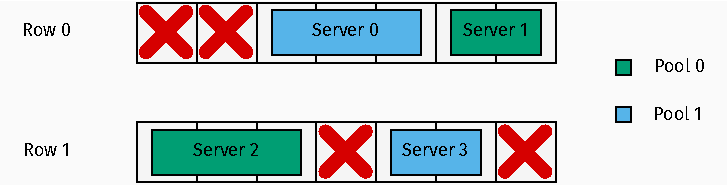
\includegraphics[width=0.9\textwidth,keepaspectratio]{../assets/dc/dc-slides.pdf}
    \caption{Example Data Center Layout}
  \end{figure}
\end{frame}

\begin{frame}{Objective}
  \begin{block}{Guaranteed Capacity}
    Given a resource pool ($p \in \mathcal{P}$), the guaranteed capacity $gc_{p}$ is a measure
    of the remaining computing capacity available in the event that at most one
    arbitrary row ($r \in \mathcal{R}$) of the data center becomes inoperable.
    \begin{equation*}
      {gc}_{p} = \min_{r \in \mathcal{R}} \left({\sum_{s \in p} c_{s}} - {\sum_{s \in p \wedge s \in r} c_{s}}\right)
    \end{equation*}
  \end{block}

  \begin{alertblock}{Objective Function}
    The objective function to be maximized is:
    \begin{equation*}
      f(s) = \min_{p \in \mathcal{P}} \left({gc}_{p}\right)
    \end{equation*}
  \end{alertblock}
\end{frame}

\begin{frame}{Example --- Solution Evaluation}
  \begin{table}[ht]
    \centering
    \begin{tabular}{@{\extracolsep{4pt}}ccccc}
      \toprule
      Pool & Row 0 & Row 1 & Guaranteed Capacity & \textbf{Score}              \\ \midrule
      0    & 5     & 10    & 5                   & \multirow{2}{*}{\textbf{2}} \\
      1    & 2     & 3     & 2                   &                             \\ \bottomrule
    \end{tabular}
    \caption{Guaranteed Capacities and Score}
  \end{table}

  \begin{figure}[h]
    \centering
    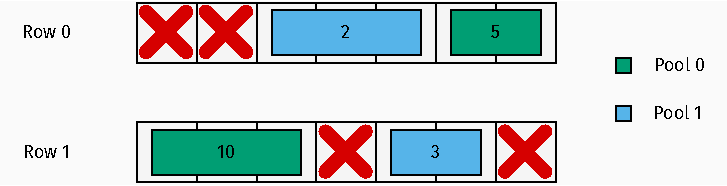
\includegraphics[width=0.9\textwidth,keepaspectratio]{../assets/dc/dc-slides-capacity.pdf}
    \caption{Example Data Center Layout (Capacities Only)}
  \end{figure}

\end{frame}

\begin{frame}{Instance Parameters}
  The \alert{problem} statement guarantees that the generated instances have the
  following properties:
  \begin{itemize}
    \item $ 1 \leq \mathcal{R} \leq 1000$: Number of rows in the data center.
    \item $ 1 \leq \mathcal{S} \leq 1000$: Number of slots in a row.
    \item $ 0 \leq \mathcal{U} \leq \mathcal{R} \times \mathcal{S}$: Number of unavailable slots.
    \item $ 1 \leq \mathcal{P} \leq 1000$: Number of resource pools to be created.
    \item $ 1 \leq \mathcal{M} \leq \mathcal{R} \times \mathcal{S}$: Number of servers to be allocated.
  \end{itemize}
\end{frame}

\begin{frame}{Decision Space}
  A \alert{solution} is a set of assignments of servers to rows and pools that does not
  violate the problem's constraints.

  A \alert{solution}, either \emph{empty}, \emph{partial}, or \emph{complete} is always
  \emph{feasible} provided that it does not violate the problem's constraints.

  \begin{itemize}
    \item \textbf{Empty Solution}: All pools and servers are unassigned.
    \item \textbf{Partial Solution}: Some servers are available and there is space for placement.
    \item \textbf{Complete Solution}: There is no space available for server placement or all the
          servers have already been assigned.
  \end{itemize}

  A \alert{component} is defined as a tuple containing the server, segment, and pool.
  \begin{itemize}
    \item A ``segment'' in the context of this problem is a contiguous sequence of slots
          that may exist in a given row.
  \end{itemize}

\end{frame}

\begin{frame}{Construction Rules}
  For constructing a solution the following \alert{rules} must be considered:
  \begin{itemize}
    \item A server can be placed in any segment that can hold its size.
    \item A server can be assigned to any resource pool available.
  \end{itemize}

  A possible \alert{heuristic construction} abiding by these rules undergoes the following steps:
  \begin{enumerate}
    \item Select an available \textbf{server} with the best capacity-to-size ratio.
    \item Select the \textbf{pool} with the lowest guaranteed capacity.
    \item Select the \textbf{row} with the least capacity for this pool that has space available.
    \item Select any \textbf{segment} in that row that can hold the server.
    \item Assign the \emph{server} to the selected \emph{segment} and \emph{pool}.
  \end{enumerate}
\end{frame}

\begin{frame}{Upper Bound}
  The construction of the upper bound is made in two steps:
  \begin{enumerate}
    \item \textbf{Row-Wise Bound} \\
          Let,
          \begin{itemize}
            \item $\Theta_{\mathcal{R} \setminus r}$: Denote the remaining empty
                  space in all the rows in the data center but the row $r$.
            \item $\sum_{\Theta_{\mathcal{R} \setminus r}}$: Denote the maximum
                  sum of the capacities of the available servers that can be
                  fractionally placed into $\Theta_{\mathcal{R} \setminus r}$ w.r.t to
                  the ratio between the capacity and the size of the server.
          \end{itemize}
          Then, the row-wise upper bound is expressed by:
          \begin{equation*}
            \Phi_{ub}^{r} = \frac{\sum_{\Theta_{\mathcal{R} \setminus r}}}{\mathcal{P}}
          \end{equation*}
    \item \textbf{Upper bound} \\
          The upper bound for a given solution $s \in \mathcal{S}$ can then be calculated as:
          \begin{equation*}
            \Phi_{ub}(s) = \min_{r \in \mathcal{R}} \Phi_{ub}^{r}
          \end{equation*}
  \end{enumerate}
\end{frame}

\begin{frame}{Upper Bound}

  Some remarks must be made on the ``\alert{Row-Wise Bound}'' $\Phi_{ub}^{r}$ calculation:
  \begin{itemize}
    \item Discarding a row involves subtracting the capacities of servers in
          the respective resource pools.
    \item If $\Phi_{ub}^{r} > gc_{p}$ for any pool $p \in \mathcal{P}$, the following correction is applied:
          \begin{enumerate}
            \item Remove relevant pools and servers.
            \item Recompute $\Phi_{ub}^{r}$ with a reduced server set and number of pools.
            \item Repeat this process until no further correction is required.
          \end{enumerate}
  \end{itemize}


\end{frame}

\begin{frame}{Results}
  We were able to achieve a score of \alert{386 points} (maximum known is 407)
  on the instance that was available, which places us at \alert{$25^{th}$ place}
  (out of 230) in the classification table.

  \vspace{0.2cm}

  This was achieved with a simple \alert{constructive search approach}, and without
  considering yet local search.
\end{frame}

\begin{frame}[fragile]{Results}
  \begin{center}
    \scalebox{0.65}{% 
      \begin{algorithm}[H]
        \DontPrintSemicolon
        \caption{Narrow Guided Heuristic Construction}
        \KwIn{Problem Instance ($\mathcal{P}$), Limit (${N}$).}
        \KwOut{Best solution ($s^{*}$).}
        \Begin{
          $s^{*} \gets \emptyset$\;
          \While{True}{
            \texttt{updated} $\gets False$\;
            $s^{\prime} \gets s^{*}$\;
            $c^{*} \gets \emptyset$\;
            \For{$i = 0$ \texttt{to} $N$}{
              $c^{\prime} \gets $ \texttt{HeuristicMoveWOR($s^{*}$, \texttt{ADD})}\;
              \texttt{ApplyMove($c^{\prime}$, $s^{\prime}$, \texttt{ADD})}\;
              \If{$\Phi_{ub}(s^{\prime})$ > $\Phi_{ub}(s^{*})$}{
                $c^{*} \gets c^{\prime}$\;
                \texttt{updated} $ \gets True$\;
              }
              \texttt{ApplyMove($c^{\prime}$, $s^{\prime}$, \texttt{REMOVE)}}\;
            }
            \If{$\lnot$ updated}{
              \Return{$s^{*}$};
            }
            \texttt{ApplyMove($c^{*}$, $s^{*}$, \texttt{ADD})}\;
          }
        }
      \end{algorithm}
    }
  \end{center}
\end{frame}

\section{Work Plan}

\begin{frame}[fragile]{Work Plan}

  The table below outlines the tasks to be executed in the upcoming semester,
  based on the objectives for this work:

  \begin{table}[ht]
    \begin{tabular}{cc}
      \toprule
      \textbf{Task} & \textbf{Description}                     \\
      \midrule
      HC\#01        & Modelling ``Optimize a Data Center''     \\
      HC-AS         & Hash Code Problem Analysis and Selection \\
      HC\#02        & Modelling Hash Code Problem \#2          \\
      HC\#03        & Modelling Hash Code Problem \#3          \\
      MH            & Meta-Heuristic Implementation            \\
      EA            & Experimental Analysis                    \\
      TW            & Thesis Writing                           \\
      \bottomrule
    \end{tabular}
    \caption{Task List}
  \end{table}
\end{frame}

\begin{frame}[fragile]{Timeline}
  \begin{figure}[fhtb]
    \centering
    \scalebox{0.6}{% 
      \begin{ganttchart}[expand chart=1.65\textwidth,hgrid,x unit=4mm, time slot
          format=isodate,time slot unit=day]{2023-02-01}{2023-07-00}
        \gantttitlecalendar{year, month=shortname} \\
        \ganttbar[bar/.append style={fill=mDarkTeal}]{HC\#01}{2023-02-01}{2023-02-21}  \\
        \ganttbar[bar/.append style={fill=mDarkTeal}]{HC-AS}{2023-02-01}{2023-02-21}  \\
        \ganttbar[bar/.append style={fill=mDarkTeal}]{HC\#02}{2023-02-15}{2023-03-28}  \\
        \ganttbar[bar/.append style={fill=mDarkTeal}]{HC\#03}{2023-03-22}{2023-05-02}  \\
        \ganttbar[bar/.append style={fill=mDarkTeal}]{MH}{2023-03-06}{2023-05-19} \\
        \ganttbar[bar/.append style={fill=mDarkTeal}]{EA}{2023-05-01}{2023-06-01} \\
        \ganttbar[bar/.append style={fill=mDarkTeal}]{TW}{2023-05-22}{2023-07-00}
      \end{ganttchart}
    }
    \caption{Project Timeline}
  \end{figure}
\end{frame}

\begin{frame}[standout]
  \talknote{Thank the audience for being awake.}
  Questions?
\end{frame}

\appendix

\section{References}

\begin{frame}[allowframebreaks]{References}
  \printbibliography[heading=none]
\end{frame}

\end{document}
